\documentclass{beamer}

\usepackage[utf8]{inputenc}
\usepackage{hyperref}

\usetheme{Berkeley}
\beamertemplatenavigationsymbolsempty
\setbeamertemplate{headline}{}
 
\title{Geo-Visualization in FoodChain-Lab}
\date{}
 
\begin{document}
\maketitle

\section{Tasks}
\begin{frame}
	\begin{itemize}
		\item Use the following workflow: \url{https://github.com/SiLeBAT/BfROpenLabResources/raw/master/GitHubPages/workflows/FCL_Example.zip}.
		\item Visualize the delivery network in the GIS mode of the \textbf{Tracing View}.
		\item Select all stations in Poland and check out where these stations are located in the Graph mode.
	\end{itemize}
\end{frame}
 
\section{1}
\begin{frame}
	\begin{center}
  		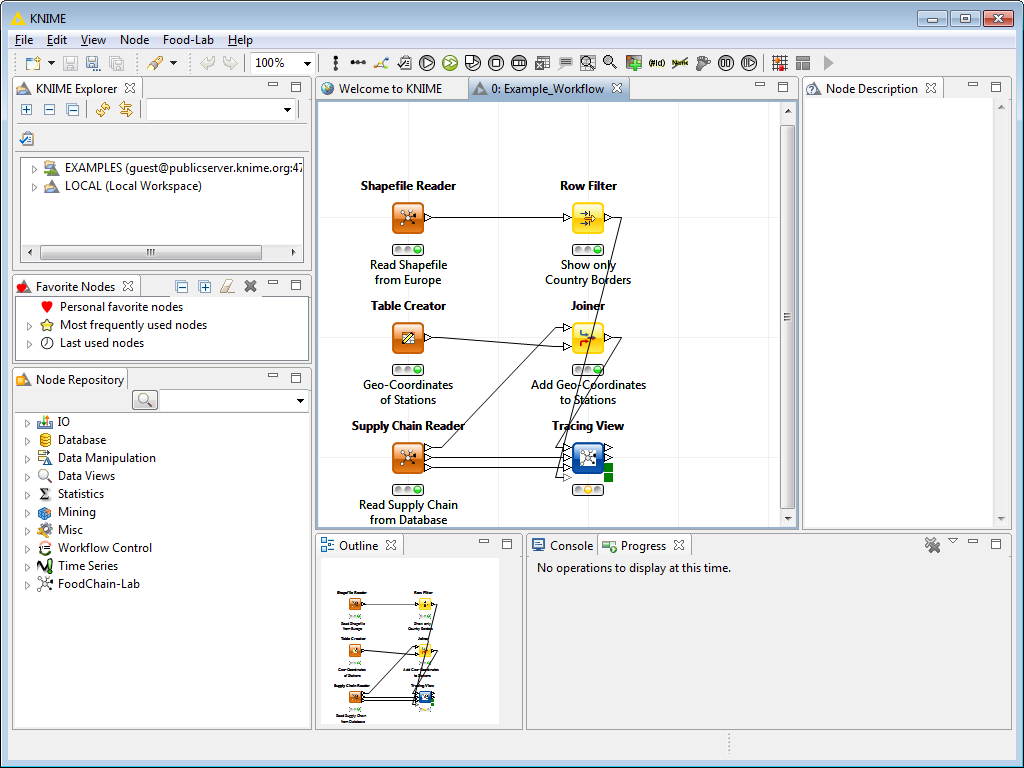
\includegraphics[height=0.6\textheight]{1.png}
	\end{center}
	\begin{itemize}
		\item Import the Example Workflow from \url{https://github.com/SiLeBAT/BfROpenLabResources/raw/master/GitHubPages/workflows/FCL_Example.zip}.
		\item Open the \textbf{Tracing View} by double-clicking on it.
	\end{itemize}
\end{frame}

\section{2}
\begin{frame}
	\begin{center}
  		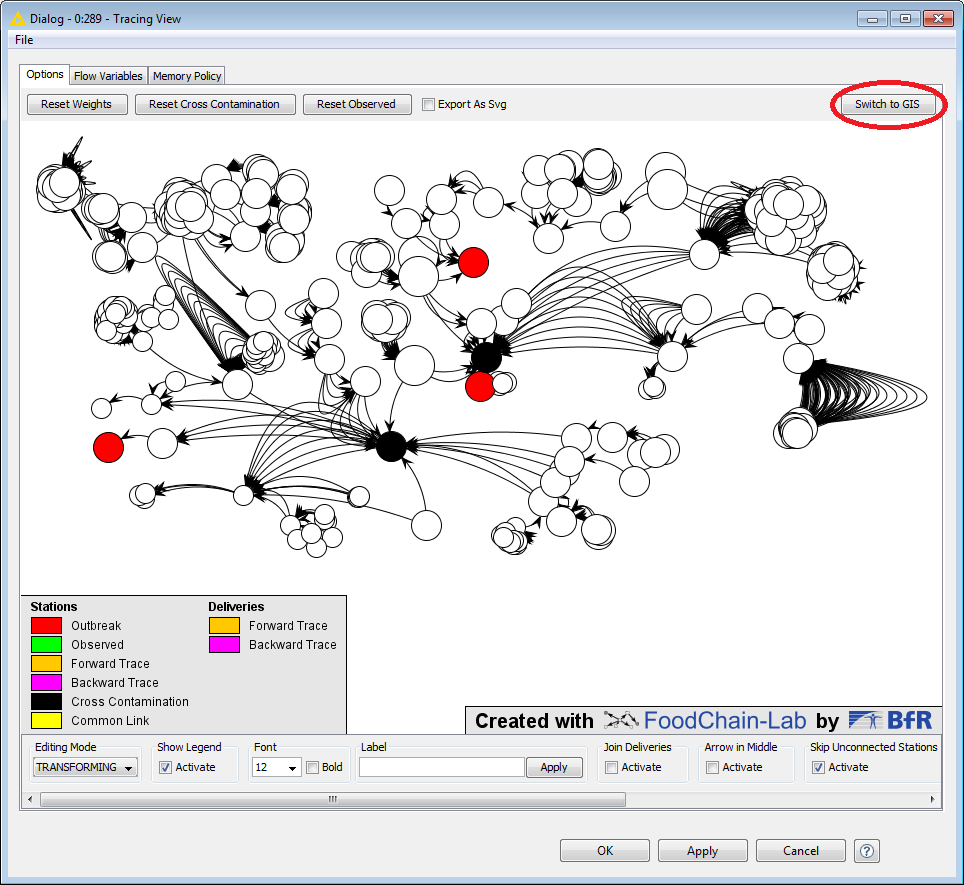
\includegraphics[height=0.6\textheight]{2.png}
	\end{center}
	\begin{itemize}
		\item Now you should see a graphical representation of the delivery network.
		\item To switch to the geographical representation click \textbf{Switch to GIS} in the upper right corner.
	\end{itemize}
\end{frame}

\section{3}
\begin{frame}
	\begin{center}
  		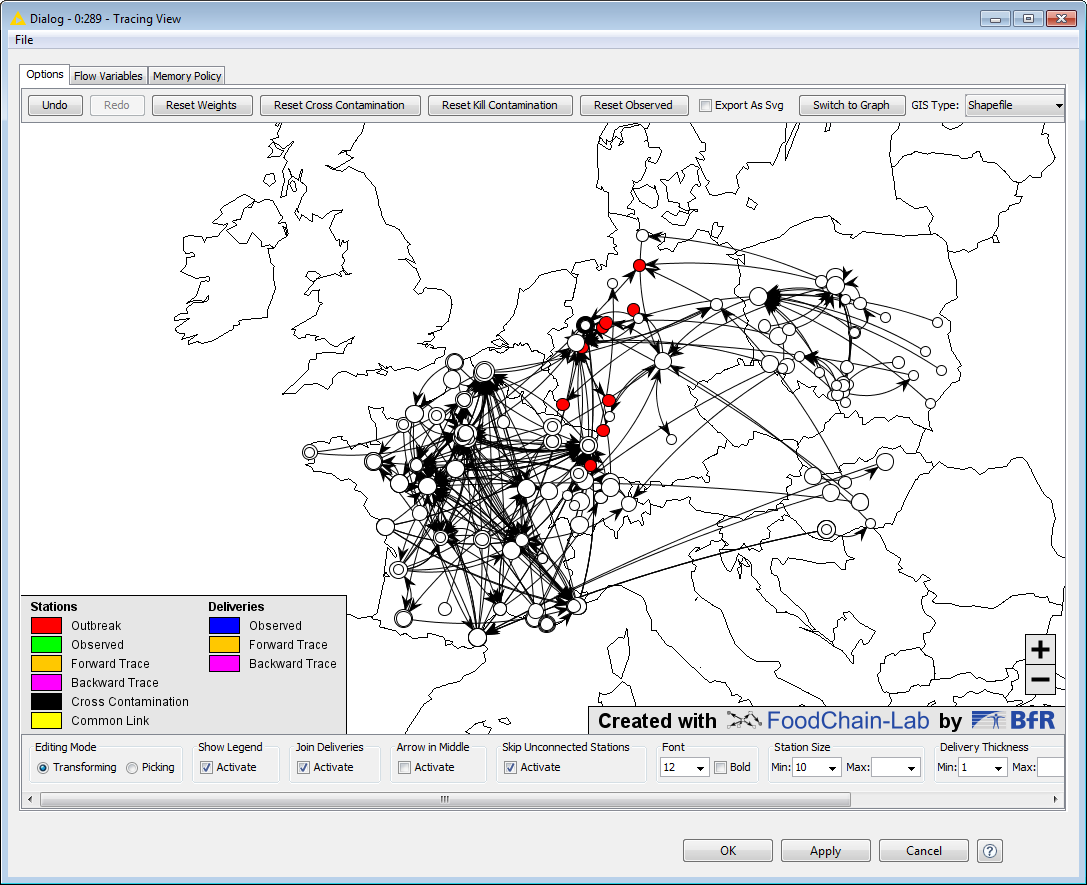
\includegraphics[height=0.6\textheight]{3.png}
	\end{center}
	\begin{itemize}
		\item The country borders, which where read from a shapefile, are used for geographical visualization.
		\item To zoom to a certain area of the graph select "Transforming" as \textbf{Editing Mode} and zoom/move the graph by using the mouse wheel and the left mouse button (works as in Google Maps).
		\it
	\end{itemize}
\end{frame}

\section{4}
\begin{frame}
	\begin{center}
  		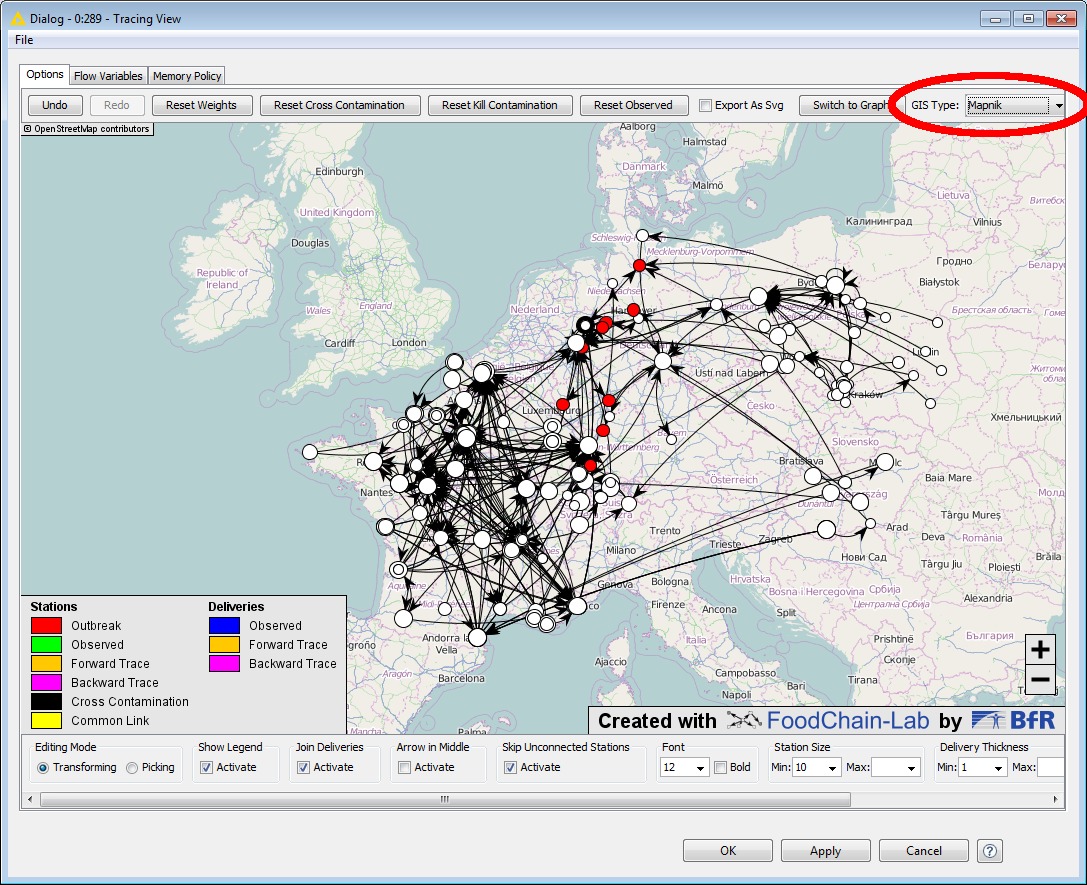
\includegraphics[height=0.6\textheight]{4.png}
	\end{center}
	\begin{itemize}
		\item If you are online, you can change the type of visualization.
		\item Select e.g. "Mapnik" as \textbf{GIS Type}.
		\item Now you should see a visualization with OpenStreetMap data.
	\end{itemize}
\end{frame}

\section{5}
\begin{frame}
	\begin{center}
  		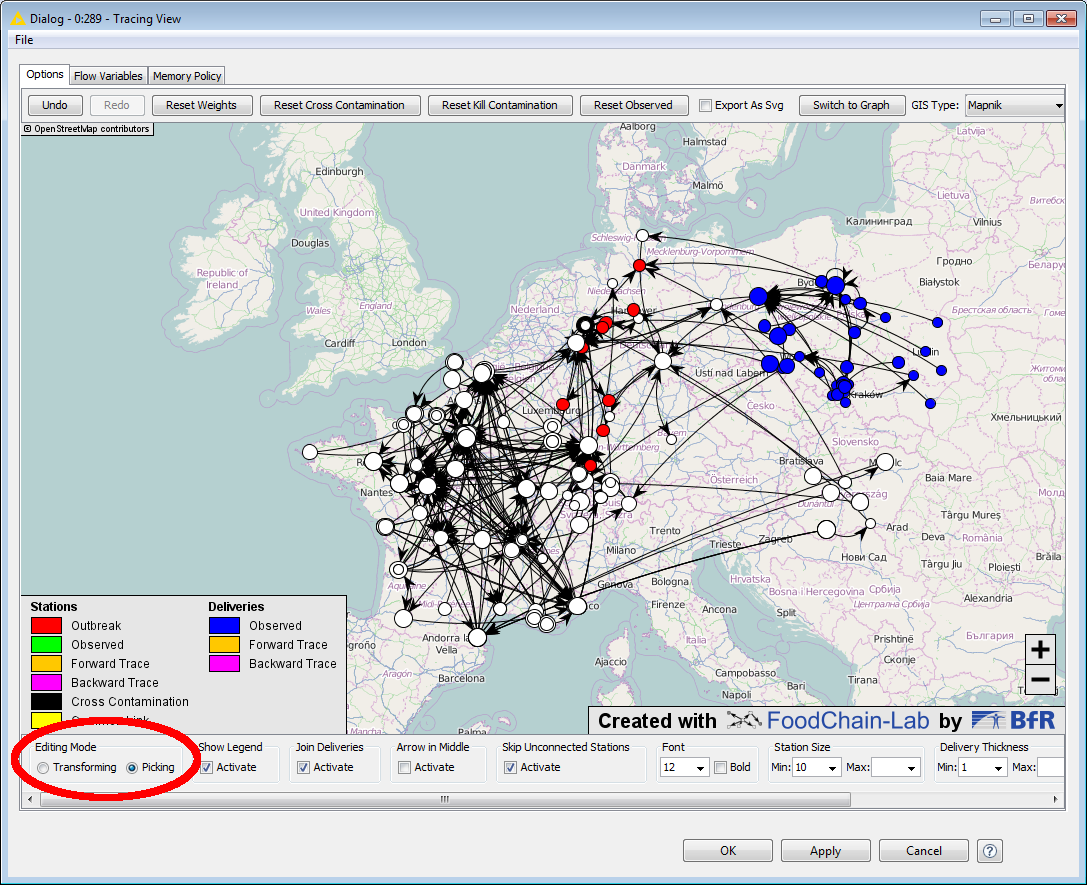
\includegraphics[height=0.55\textheight]{5.png}
	\end{center}
	\begin{itemize}
		\item We can now select certain stations based on geography.
		\item Select "Picking" as \textbf{Editing Mode} and select all stations in Poland by dragging with the left mouse button a rect around the stations.
		\item The selected stations are now colored blue.
		\item Switch back to the graphical view by clicking \textbf{Switch to Graph} in the upper right corner.
	\end{itemize}
\end{frame}

\section{6}
\begin{frame}
	\begin{center}
  		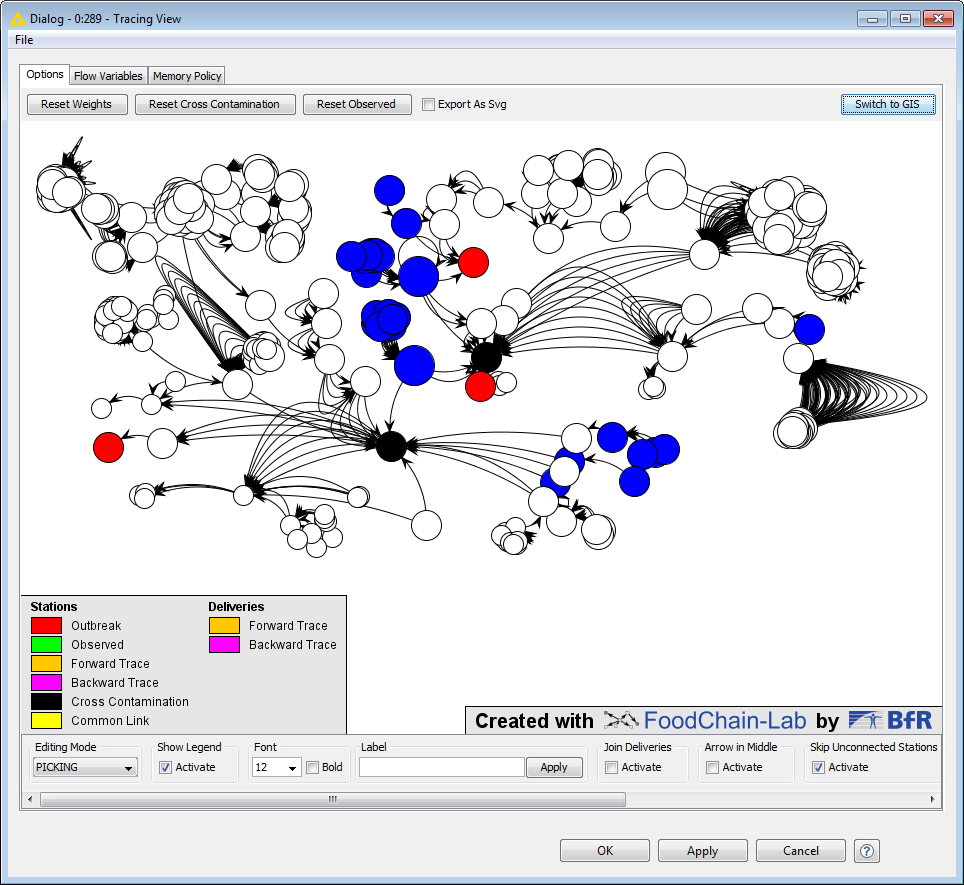
\includegraphics[height=0.6\textheight]{6.png}
	\end{center}
	\begin{itemize}
		\item The blue stations are the ones you selected in the geographical view, since changes you make in any of the view are automatically applied to the other view.
		\item That makes it easy to switch back and forth between both representations and use the benefits of both.
	\end{itemize}
\end{frame}

\section{7}
\begin{frame}
	\begin{center}
  		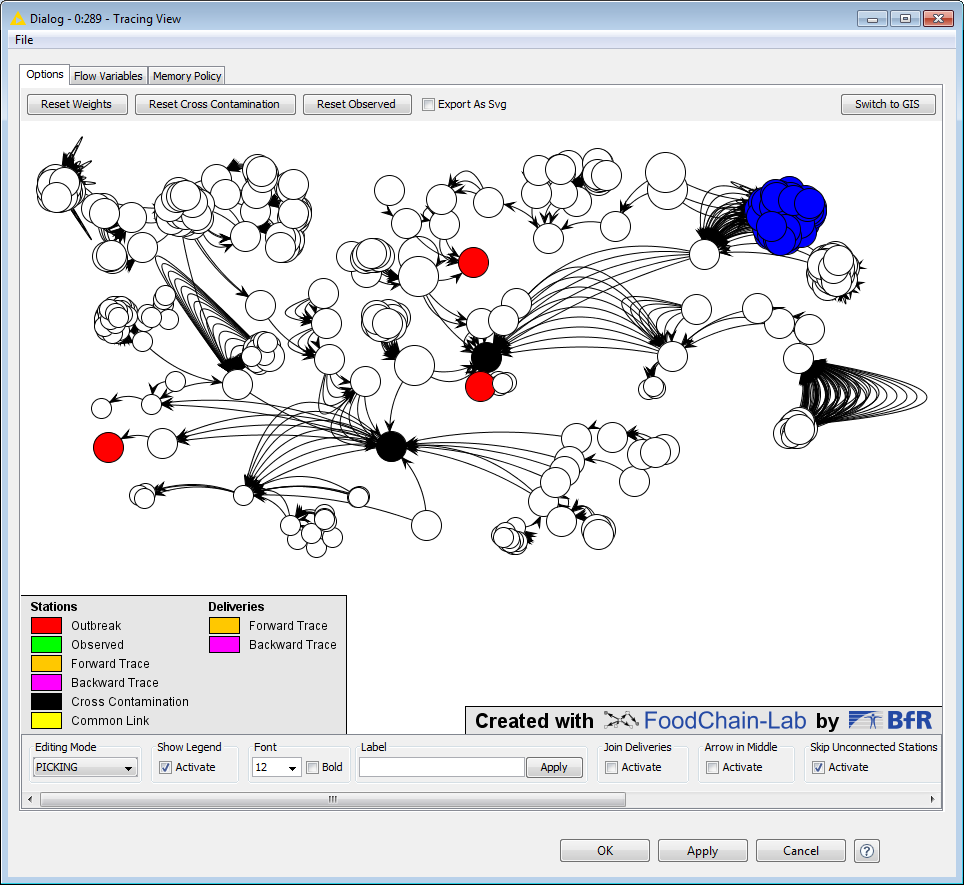
\includegraphics[height=0.6\textheight]{7.png}
	\end{center}
	\begin{itemize}
		\item Lets now select a certain "cluster" in the graphical view and see where the stations are in the geographical view.
		\item So select the "cluster" in the red circle and click \textbf{Switch to GIS}.
	\end{itemize}
\end{frame}

\section{8}
\begin{frame}
	\begin{center}
  		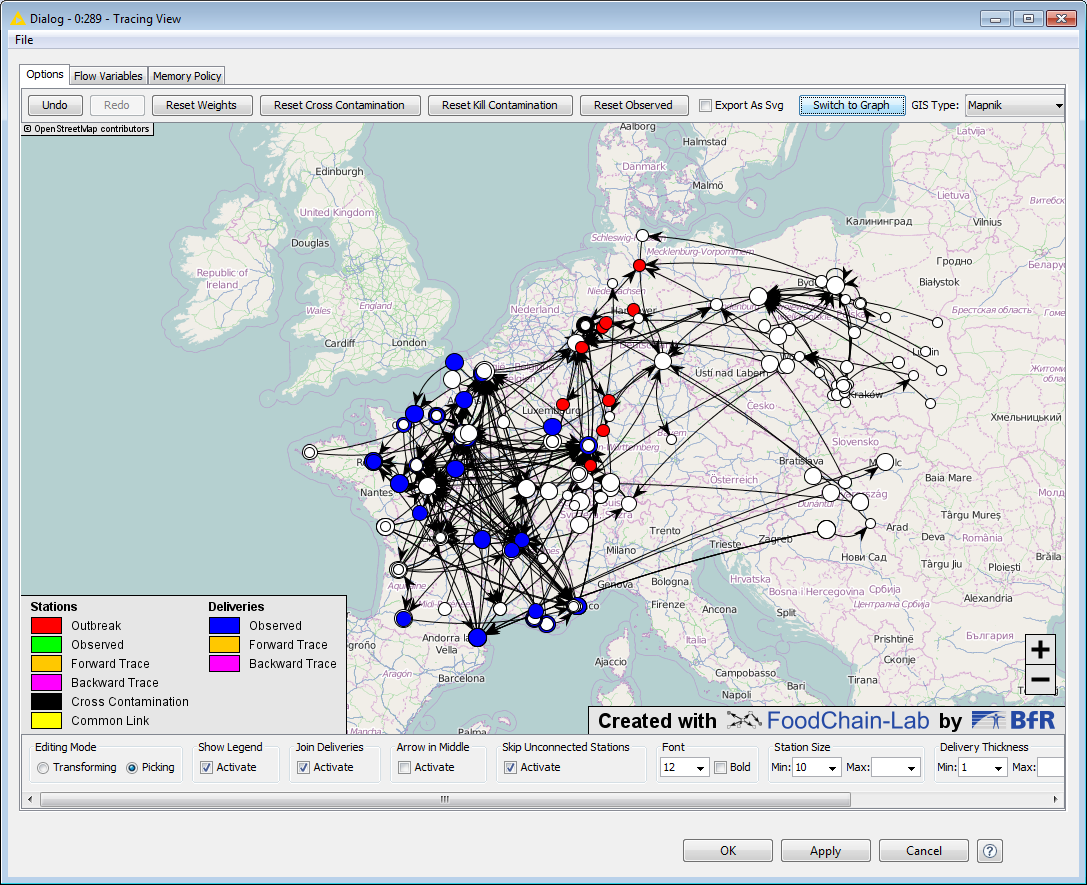
\includegraphics[height=0.6\textheight]{8.png}
	\end{center}
	\begin{itemize}
		\item As you can see the stations of the cluster are located all over France.
	\end{itemize}
\end{frame}

\end{document}